\subsubsection{UC13 - Storico prenotazioni}
 \begin{figure}[h]
	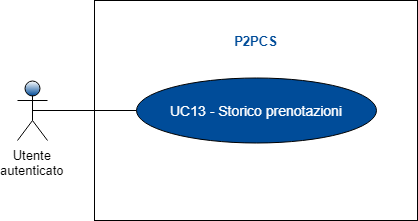
\includegraphics[width=8cm]{res/images/Schemagenerale4.png}
	\centering
	\caption{UC13 - Storico prenotazioni}
\end{figure}
\begin{itemize}
	\item \textbf{Attori Primari}: utente autenticato;
	\item \textbf{Descrizione}: agli utenti autenticati è resa disponibile una maschera che presenta la lista di tutte le sue prenotazioni concluse dalla quale si possono ricavare le seguenti informazioni:
	\begin{itemize}
		\item marca;
		\item modello;
		\item data;
		\item ora;
		\item nome del proprietario;
		\item anno d'immatricolazione.
	\end{itemize} 
	\item \textbf{Scenario principale}: l'utente visualizza la lista contenente tutte le sue prenotazioni concluse;
	\item \textbf{Precondizione}: l'utente autenticato ha selezionato la voce \textit{Storico prenotazioni} dal menu dell'applicazione;
	\item \textbf{Post-condizione}: l'utente autenticato ha visualizzato lo storico delle sue prenotazioni concluse. 
\end{itemize} 
